\section{Friday, October 25, 2019}

\subsection{Algorithmic Complexity}

\subsubsection{Time Functions and Big-$\O$ Notation}
While we have already looked at the basics of Big-$\mathcal{O}$ notation, we will now learn how to analyze programs and determine their asymptotic complexity on our own. 

The \vocab{critical section} of a program is another word for the ``heart" of an algorithm. In essence, it indicates the portion of code where the most ``work" is performed in terms of time needed. The critical section of an algorithm dominates its overall execution time, and its operation is central to the functioning of a program. Typically, the sources of a critical section comes from loops or recursion.

Our goal is to find the asymptotic complexity of various algorithms. The general approach for doing so is ignoring frequently executed parts of the algorithm, finding the critical of the algorithm, and determining how many times the critical section is executed as a function of the problem size. 


Here's an example of some code in which we can easily identify the critical section:

\begin{lstlisting}
A
for (int i = 0; i < n; i++) {
    B /* This is the critical section. */
}
C
\end{lstlisting}

Suppose $A$, $B$, and $C$ are sequences of constant-time operations (for example, print statements). Then, $A$ is executed exactly once, $B$ is executed $n$ times (it is inside of a loop that loops through $n$ times), and $C$ is executed exactly once. Therefore, the total number of operations we perform is $T(n) = 1 + n + 1 = n + 2$. The high-order term of $T(n)$ is $n$, which implies that this algorithm runs in $\O(n)$ time. The function $T(n)$, which gives the exact number of operations, is referred to as our \vocab{time function}. Using this terminology, our asymptotic complexity is the high-order term of our time function. \\

It is important to be able to compute the time function exactly. Thus, it is important to be careful, particularly with the bounds of our loops. In the previous example, it is clear that the loop iterates through exactly $n$ times (once for $i = 0$, once for $i = 1$, all the way up to $i = n - 1$). If we instead wrote our loop as \verb!for (int i = 1; i <= n; i++)!, then our loop would still iterate through $n$ times. But \verb!for (int i = 0; i <= n; i++)! iterates through $n + 1$ times. Another example of a for-loop is given by \verb!for (int i = 0; i < n; i += n)!, which executes only once. \\


Here's another example:

\begin{lstlisting}
A
for (int i = 0; i < n; i++) {
    B
    for (int j = 0; j < n; j++) {
        C
    }
}
D
\end{lstlisting}

Once again, suppose $A, B, C, D$ are sequences of constant-time operations. In this scenario, $A$ is executed exactly once. $B$ is executed exactly $n$ times (it is in a for-loop that iterates through $n$ times), $C$ is executed $n^{2}$ times (it is inside a for-loop that executes another for-loop that iterates $n$ times exactly $n$ times, so we have $n \cdot n = n^{2}$ executions).  Finally, $D$ is executed once. Therefore, our time function is given by
\[
T(n) = 1 + n + n^{2} + 1 = n^{2} + n + 2.
\]

The high-order term of $T(n)$ is $n^{2}$, so this algorithm runs in $\O(n^2)$ time.  \\

Here is a third example:

\begin{lstlisting}
A
for (int i = 0; i < n; i++) {
    for (int j = i + 1; j < n; j++) {
        B /* Critical section. */
    }
}
\end{lstlisting}

Here, $A$ is executed exactly once. But now, the inner for-loop depends on the value of the outer for-loop. How do we determine the number of times $B$ is executed? We can note that when $i = 0$, the inner for-loop starts at $j = 1$, and it goes up to $n$. This contributes a total of $(n - 1)$ executions. Next, when $i = 1$, the inner for-loop starts at $j = 2$, and goes up to $n$. This contributes a total of $(n - 2)$ executions. This process continues up until the inner for-loop contributes $0$ executions. Therefore, our time function is given by
\begin{align*}
T(n) &= \underbrace{1}_{\text{Executions of Statement $A$}} + \underbrace{\left((n - 1) + (n - 2) + \cdots + 1 + 0\right)}_{\text{Executions of Statement $B$}} \\[1em]
&= 1 + \frac{n(n - 1)}{2} \\[1em]
&= \frac{n^2}{2} - \frac{n}{2} + 1
\end{align*}

\noindent where we used the identity $\sum_{k=1}^{n} k = n(n + 1)/2$ to simplify the number of executions of Statement $B$. Since the high-order term of of $T(n)$ is $n^2$, we conclude our algorithm is $\O(n^{2})$. 

\noindent It is important to note that minor changes to algorithms won't affect the asymptotic complexity of the algorithm. For example, if we instead looped from $i = 0$ and $j = i + 1$ up to $n/2$ instead of $n$, our algorithms would still be $\O(n^2)$ (although, our time functions would decrease). Essentially, Big-$\O$ notation is mostly concerned with \textit{long-run} behavior, whereas time functions are concerned with exact behavior. \\

Here is another example:

\begin{lstlisting}
int i = 1;
while (i < n) {
    /* This is the critical section. */
    A
    i = 2 * i;
}
B;
\end{lstlisting}

\noindent In this case, the statement $i = 1$ contributes $1$ to our time function (the time function accounts for \textit{every} operation). Now, how many times does $A$ execute? The answer is $\log_{2}(n)$. This can be seen easily by plugging in different powers of $2$ for $n$, and tracing the code. Logarithmic time complexity typically indicates that we are increasing the loop variable by some constant factor, or we're reducing the problem at-hand by a constant factor. Thus, statement $A$ contributes a $\log_2(n)$ term to our time function, and the re-assignment of $i$ inside of the for-loop contributes another $\log_2(n)$ term. Finally, the statement $B$ executes one more operation, from which we obtain
\[
T(n) = 1 + \log_2(n) + \log_2(n) + 1 = 2(\log_2(n) + 1).
\]

\noindent The high-order term here is $\log(n)$ so we conclude that this algorithm is $\O(\log(n))$. \\

\subsection{Complexity of Recursive Algorithms}

How can we compute the complexity of a recursive algorithm? We can do this by writing the recurrence in terms of itself. For example, consider the following program:

\begin{lstlisting}
int fact(n) {
    if (n == 0) return 1;
    return n * fact(n - 1);
}
\end{lstlisting}

If $n$ is greater than $0$, then we perform exactly $3$ operations and perform a recursive call on $n - 1$. On the other hand, if $n$ is equal to $0$, then we perform only one operation. In this case, our time function can be expressed by $T(n) = T(n - 1) + 3$ with base case $T(1) = 0$. This type of equation is known as a \vocab{recurrence}. There are many ways to solve recurrences, but knowing how to solve them is not necessary in this class. \\

\noindent By performing iteration, we can solve the recurrence in a very informal way by identifying a pattern:

\begin{align}
T(n) &= T(n - 1) + 3 \\
&= T(n - 2) + 6 \\
&= T(n - 3) + 9 \\
&= \ldots \\
&= T(n - k) + 3k.
\end{align}

We keep on iterating until $k = n$ in which case we obtain $T(n) = T(0) + 3n$. But since we have the base case $T(0) = 1$, we find $T(n) = 3n + 1$. Therefore, we can conclude that the algorithm runs in$\O(n)$ time. \\


Here's another example of an algorithm (pseudocode is shown):

\begin{lstlisting}
MergeSort(Array) {
    if (n == 1) return;
    MergeSort(first half of array)
    MergeSort(second half of array)
    Merge the two halves. /* Requires n operations. */
}
\end{lstlisting}

In this algorithm, we perform $n$ operations per recursive call. In addition, we make two calls to the algorithm with subproblem size $n/2$, so we obtain $T(n) = 2T(n/2) + n$ as our recurrence equation. The base case occurs when $n = 1$ in which case we perform just one operation. Thus, our base case is given by $T(1) = 1$.  This recurrence can be a little bit more tricky to solve, but the solution's high order term is $n\log_{2}(n)$. Thus, this algorithm runs in $\O(n\log(n))$ time. 


\subsection{Additional Complexity Measures}

So far, we have only discussed Big-$\O$ notation, which is an upper bound on the number of operations we perform. However, we can also use Big-$\Omega$ notation, which is a \textit{lower} bound on the number of operations we perform (e.g. what is the least number of operations we perform?). \\

\noindent Suppose we want to find the maximum element in an array with $n$ numbers. One easy way to do this is to keep track of the maximum value seen so far, and update this value when we see a new maximum. This algorithm runs in $\O(n)$ time. But, it can also be shown that a lower bound for this algorithm is $\Omega(n)$ time. This is true because there cannot exist an algorithm that finds the maximum of $n$ numbers without at least looking at what the $n$ numbers are. But even the act of just looking at the $n$ numbers requires linear time. \\

When the Big$-\O$ and Big-$\Omega$ of an algorithm are equal (i.e. $\Omega(f(n)) = \O(f(n))$ for some function $f(n)$), then we say that the algorithm is $\Theta(f(n))$. This is a stronger result. 


\subsection{Trees}
A \vocab{tree} is a hierarchical, non-linear data structure that can be used to represent a one-to-many relationship between elements. The data structure consists of a \vocab{root node} which is typically the topmost node in a data structure as well as many other \vocab{internal nodes}. Each node stores values and references to other nodes in the tree. Below is an example of a tree:

\begin{figure}[h]
\centering
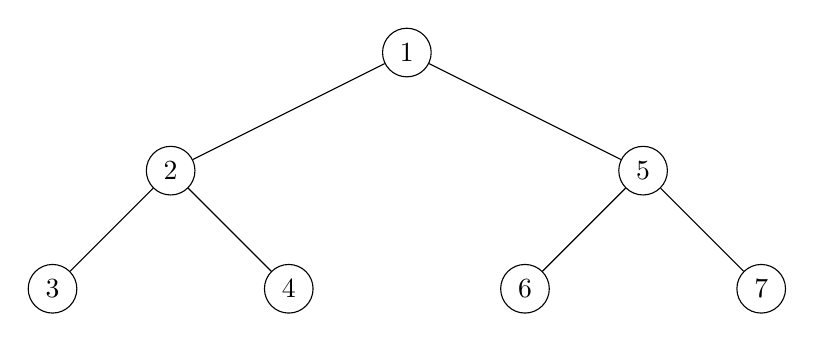
\begin{tikzpicture}[level/.style={sibling distance=60mm/#1}]
\node [circle,draw] (z){$1$}
  child {node [circle,draw] (a) {$2$}
    child {node [circle,draw] (b) {$3$}
    }
    child {node [circle,draw] (g) {$4$}}
  }
  child {node [circle,draw] (j) {$5$}
    child {node [circle,draw] (k) {$6$}
    }
  child {node [circle,draw] (l) {$7$}}
};
\end{tikzpicture}
\caption{An Example of a Tree}
\end{figure}

Here, the node labelled $1$ is the root node, and every other node is an internal node. 

What are trees useful for? Trees are good for clearly depicting relationships. For example, we can model ancestry trees, or relationships between people. We can also model a network of cities with vertices representing cities, and an edge between two cities representing a roadway or path between the two cities.

In the diagram above, we see that every node other than $3, 4, 6$ and $7$ have two nodes coming out, underneath them. We call these nodes the \vocab{child nodes} of the node that they are coming out of (so nodes $3$ and $4$ are the children of node $2$, and node $7$ has no children). Also, we can differentiate between the two children by using the terminology \vocab{left child} and \vocab{right child}. 

The \vocab{level} of a node is a measure of the node's distance from the root. More precisely, if the node is the root of the tree, then its level is $1$. Otherwise, its level is its parent's level plus one. The \vocab{height} of a tree is the maximum level of any node in the tree. \\

A \vocab{binary tree} is a special kind of tree in which each node has at most $2$ children. We will place a special focus on this type of tree, starting next lecture. 